\documentclass[a4paper,14pt]{extarticle}
\usepackage{extsizes}
\usepackage{multicol}
\usepackage{amsmath}
\usepackage{float}
\usepackage{hyperref}
\usepackage{graphicx}
\graphicspath{ {./images} }
\usepackage[margin=1in]{geometry}
\title{Fisica}
\author{}
\date{Aprile 2024}

\begin{document}

% \begin{NoHyper}
\maketitle
\tableofcontents
\newpage

\section{Formule}


\begin{enumerate}

\item Arrangement of the principal measurements in physics

\begin{figure}[H]
\centering
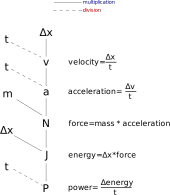
\includegraphics[width=0.5\textwidth]{arrangements.pdf}
\end{figure}


\begin{itemize}
\item $v$ = $\frac{m}{s}$
\item $a$ = $\frac{m}{s^2}$
\item $N$ (Newton) = $Kg\frac{m}{s^2}$
\item $J$ (Joule) = $N*m=Kg\frac{m^2}{s^2}$
\item $W$ (Watt) = $\frac{J}{s}=Kg\frac{m^2}{s^3}$
\end{itemize}


\item \textbf{Gravitational potential energy}: the energy an object possesses because of its position in a gravitational field.

The most common use of gravitational potential energy is for an object near the surface of the Earth where the gravitational acceleration can be assumed to be constant at about 9.8 m/s2.

\begin{equation}
\Delta U=mg\Delta h
\end{equation}

Where:

\begin{enumerate}
\item[$\Delta U$] is the change in gravitational energy
\item[$m$] is the mass
\item[$g$] is the gravity
\item[$\Delta h$] is the change in height
\end{enumerate}

\item Displacement of an object thrown vertically

\begin{equation}
s=ut-\frac{1}{2}gt^2
\end{equation}

Where:
\begin{enumerate}
\item[$s$] is the final displacement
\item[$u$] is the initial velocity
\item[$t$] is the time passed
\item[$g$] is the gravitational constant
\end{enumerate}

\item Velocity of an object thrown vertically

\begin{equation}
v=u-gt
\end{equation}

Where:
\begin{enumerate}
\item[$v$] is the final velocity
\item[$u$] is the initial velocity
\item[$t$] is the time passed
\item[$g$] is the gravitational constant
\end{enumerate}



\end{enumerate}





\section{Esercizi}

\subsection{Moto lineare} \label{sec:motolineare}

\setcounter{equation}{0}
\begin{enumerate}

\item A speedboat has an acceleration of 2 $\frac{m}{s^2}$.  \label{ex_f_1} 

What would the final velocity of the speedboat be after 5 seconds if the initial velocity of the speedboat is 4 $\frac{m}{s}$?

( Soluzione a pagina \pageref{sol_f_1} )

\item A vehicle has an acceleration of 5 $\frac{m}{s^2}$. \label{ex_f_2} 

What would the final velocity of the vehicle be after 10 seconds if the initial velocity of the vehicle is 20 $\frac{m}{s}$?

What is the displacement of the vehicle during the 10 $s$ time interval?

( Soluzione a pagina \pageref{sol_f_2} )

\item A child on a toboggan starts from rest and accelerates down a snow-covered hill at 0.8$\frac{m}{s^2}$.  \label{ex_f_3} 

How long does it take the child to reach the bottom of the hill if it is 25.0 m away?

( Soluzione a pagina \pageref{sol_f_3} )

\item  A car accelerates uniformly from a velocity of 21.8 $\frac{m}{s}$ to a velocity of 27.6 $\frac{m}{s}$. \label{ex_f_4} 

The car travels 36.5 m during this acceleration.


What was the acceleration of the car?


Determine the time interval over which this acceleration occurred.


( Soluzione a pagina \pageref{sol_f_4} )


\item A motorcycle starts from rest and accelerates at +2.50 $\frac{m}{s^2}$ for a distance of 150.0 m. \label{ex_f_5} 



It then slows down with an acceleration of –1.50 $\frac{m}{s^2}$ until the velocity is +10.0 m/s.

Determine the total displacement of the motorcycle.


( Soluzione a pagina \pageref{sol_f_5} )


\end{enumerate}




\subsection{Power, Work, Acceleration, Mass} \label{sec:powoama}

\setcounter{equation}{0}
\begin{enumerate}
\item 
A 1200 Kg race car accelerates from rest to % 160
180 km/h in % 7.5
8 seconds.  What is the average power output of the engine?
\label{ex_f_6} 

( Soluzione a pagina \pageref{sol_f_6} )

\end{enumerate}



\subsection{Carrucole} \label{carrucole}

\subsubsection{Corpi appesi a fili}

\begin{enumerate} % corpi appesi a fili

\item % corpi appesi a fili
\label{car_x_01}
Un corpo di massa $mc = 7 kg$ è appeso al soffitto di una stanza mediante un filo di massa
$mf = 50 g$ ed è in quiete.


\begin{enumerate}
\item Trovare la forza che il corpo esercita sul filo
\item Trovare la forza che il soffitto esercita sul filo
\end{enumerate}

Soluzione a pagina \pageref{car_s_01}


\end{enumerate} % corpi appesi a fili



\subsubsection{Due Carrucole e una forza}

\begin{figure}[h]
\centering
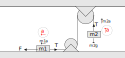
\includegraphics[width=0.8\textwidth]{carrucole.pdf}
\end{figure}

\begin{itemize}
\item $m_1=50$
\item $m_2=80$
\item $F=1N$
\end{itemize}

L'accelerazione $a$ è l'incognita che dobbiamo trovare.

Per ognuna delle due masse si genera una forza di inerzia che si oppone in senso inverso alla causa del moto.

Le forze di inerzia sono $m_1a$ e $m_{2}a$, in senso contrario all'accelerazione.

Nota bene: Durante l'impostazione del problema non è ancora chiaro quale sia il senso del moto dei vari pesi.

Non so se un peso si muove in un modo o nell'altro.

Quindi all'accelerazione incognita (in rosso) è stato assegnato un senso arbitrario, giusto per capire quale forza si oppone a quale altra e quindi dove mettere i $+$ e i $-$.

Alla fine otterrò un numero che potrà essere negativo o positivo; questo sarà il modulo della forza.

Le forze in ognuno dei due sistemi costituito da peso e corda si equivalgono; vuol dire che la loro somma è zero.

Nel primo peso la somma di queste forze deve essere zero:

\begin{enumerate}
\item $F$: la forza applicata alla prima massa
\item $m_1a$: la forza applicata dall'accelerazione risultante
\item $-T$ la tensione della corda, negativa perché tira in senso opposto
\end{enumerate}

Posso quindi scrivere che:
\setcounter{equation}{0}

\begin{equation}
\left\{
\begin{array}{ll}
F + m_1a -T = 0\\
m_2g -T - m_2a =0
\end{array}
\right.
\end{equation}

Quindi

\begin{equation}
\Rightarrow
\left\{
\begin{array}{ll}
T - F = m_1a\\
m_2g -T = m_2a
\end{array}
\right.
\end{equation}

Dalla prima ricavo $T$:


\begin{equation}
T = F + m_1a
\end{equation}

Sostituisco nella seconda

\begin{equation}
m_2g -F - m_1a = m_2a
\end{equation}

Sposto $m_1a$ a destra

\begin{equation}
m_2g -F = m_1a + m_2a
\end{equation}

Raccolgo $a$:

\begin{equation}
m_2g -F = a(m_1 + m_2)
\end{equation}

Ed ecco $a$:

\begin{equation}
a=\frac{
m_2g -F
}{
m_1 + m_2
}
\end{equation}

Ora posso sostituire i valori iniziali:

\begin{equation}
a=\frac{ m_2g -F }{ m_1 + m_2 } =  \\
\frac{80-1}{80+50} = \\
\frac{79}{130} = \\
.53846153846153846153
\end{equation}


\begin{minipage}{\textwidth}

\subsubsection{Una Carrucola e tre pesi}

\begin{figure}[H]
\centering
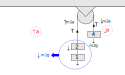
\includegraphics[width=0.8\textwidth]{carrucole.2}
\end{figure}

\begin{itemize}
\item $m_1=2 kg$
\item $m_2=4 kg$
\item $m_3=1 kg$
\end{itemize}

\end{minipage}

\begin{enumerate}
\item \textbf{Find the acceleration of the 4 kg block.}

Per quanto riguarda $a$, i pesi da 1 3 possono essere considerati come una unica massa che chiameremo $m_1$.

La forza di inerzia corrispondente è $m_1g$.

Notare il senso delle frecce nel disegno: indicano il segno delle varie forze.

per esempio $m_1g$ è diretta in basso; all'inizio abbiamo deciso arbitrariamente che $a$ vada nella direzione opposta, quindi considerando l'equazione per i pesi $1$ e $3$, se $m_1g$ ha segno positivo allora $a$ avrà segno negativo.

il sistema di equazioni è quindi:
\setcounter{equation}{0}

\begin{equation}
\left\{
\begin{array}{ll}
m_1g -T - m_1a =0 \\
m_2g + m2a -T =0
\end{array}
\right.
\end{equation}

Dalla prima ricavo $T$:

\begin{equation}
T = m_1g-m_1a
\end{equation}

Sostituisco nella seconda:


\begin{equation}
\begin{array}{ll}
m_2g+m_2a-T=0 \\
\Rightarrow
m_2g+m_2a-(m_1g-m_1a)=0 \\
\Rightarrow
m_2g+m_2a-m_1g+m_1a=0
\end{array}
\end{equation}

Raccolgo $a$:

\begin{equation}
a(m_2+m_1)=m_1g-m_2g
\end{equation}

Quindi

\begin{equation}
a=\frac{
m_1g-m_2g
}{
m_2+m_1
}
\end{equation}

Sostituendo con i valori iniziali

\begin{equation}
a=\frac{
(3-4)g
}{
3+4
}
\end{equation}

\begin{equation}
\Rightarrow
=\frac{ -1g }{ 7 }
=\frac{ -10 }{ 7 }
=-1.42857142857142857142
\end{equation}

\setcounter{equation}{0}
\begin{minipage}{\textwidth}


\item \textbf{Find the tension in the string supporting the 4-kilogram block.}

Rivediamo il disegno:

\begin{figure}[H]
\centering
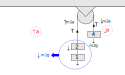
\includegraphics[width=0.8\textwidth]{carrucole.2}
\end{figure}

Sul peso $4$ agiscono queste forze:

\begin{enumerate}
\item[$m_2g$] la forza di gravità
\item[$T$] la tensione della corda
\item[$m_2a$] la forza di inerzia dell'oggetto
\end{enumerate}

La somma delle forze deve essere uguale all'accelerazione risultante.

Il senso delle forze lo conosciamo, quindi:

\end{minipage}

\begin{equation}
m_2g-T=m_2a
\end{equation}

\begin{equation}
\Rightarrow
T=m_2g-m_2a
\end{equation}

L'accelerazione $a$ l'abbiamo calcolata prima: $ a=\frac{g}{7}$

\begin{equation}
\Rightarrow
T=4*10-4*(\frac{10}{7})=34.28571428571428571429
\end{equation}

\begin{minipage}{\textwidth}
\item \textbf{Find the tension in the string connected to the l-kilogram block}

Le forze che agiscono sul peso da 1 kg (chiamiamolo $m$) sono :

\setcounter{equation}{0}
\begin{enumerate}
\item[$mg$] la forza di gravità
\item[$T$] la tensione della corda (l'incognita)
\item[$ma$] la forza di inerzia dell'oggetto
\end{enumerate}

Come prima, la somma delle forze deve essree uguale all'accelerazione risultante.

\begin{equation}
mg -T = -ma
\end{equation}

(stavolta $ma$ è negativa perché va nella direzione opposta a prima)

\begin{equation}
T=mg +ma=1*10+1*\frac{10}{7}= 11.42857142857142857142
\end{equation}

\end{minipage}
\end{enumerate}

\subsubsection{Carrucola e forza di Archimede}

\begin{figure}[h]
\centering
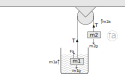
\includegraphics[width=0.8\textwidth]{carrucole.3.pdf}
\end{figure}

Calcolare l'accelerazione $a$ e la tensione della fune sapendo che :

\begin{enumerate}
\item $m1$ è uguale ad 1 kg
\item $m2$ è uguale ad 3 kg
% \item 
\item $m1$ è immerso in un liquido che da origine ad una Forza di Archimede ($Fa$) pari a 1 Newton.
\end{enumerate}

% https://www.savemyexams.co.uk/as/physics/cie/22/revision-notes/2-kinematics/2-1-equations-of-motion/2-1-9-projectile-motion/
% https://isaacphysics.org/concepts/cp_projectiles?stage=all
\subsection{Moto di proiettili}

\begin{enumerate}

\item A ball is thrown in the air with speed $12\frac{m}{s}$ at an angle of $70\circ$ to the horizontal.  \label{ex_p_1}

Draw a diagram to show where it is $1.5$ seconds later.

( Soluzione a pagina \pageref{sol_p_1} )

\item A stone is thrown from the edge of a cliff with speed $18 \frac{m}{s}$.

Draw diagrams to show the path of the stone in the next $4$ seconds if it is thrown horizontally or at $30\circ$ to the horizontal. \label{ex_p_2}

( Soluzione a pagina \pageref{sol_p_2} )

\item In a game of tennis a player serves the ball horizontally from a height of $2$ metres.\label{ex_p_3}

It has to satisfy two conditions.
\begin{enumerate}
\item It must pass over the net, which is 0.9 metres high at a distance of $12$ metres from the server
\item It must hit the ground less than 18 metres from the server
\end{enumerate}

At what speeds can it be hit?

( Soluzione a pagina \pageref{sol_p_3} )

\item A motorcycle stunt-rider moving horizontally takes off from a point $1.25 m$ above the ground, landing 10 m away. \label{ex_p_4}

\begin{figure}[H]
\centering
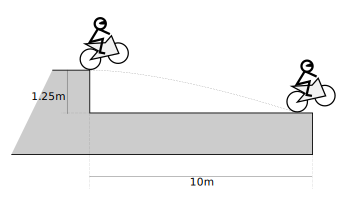
\includegraphics[width=0.8\textwidth]{moto.pdf}
\end{figure}

What was the speed at take-off?

( Soluzione a pagina \pageref{sol_p_4} )

\end{enumerate}



\subsection{Moto Circolare}

\subsubsection{Formule}

\setcounter{equation}{0}

La "\textit{Legge oraria}":

\begin{equation}
\theta=\theta_0+\omega\cdot t
\end{equation}

Frequenza e periodo:

\begin{equation}
\begin{array}{ll}
\textrm{Frequenza }f=\frac{1}{T} \\
\\
\textrm{Periodo }T=\frac{1}{f}
\end{array}
\end{equation}

Velocità angolare:

\begin{equation}
\omega=\frac{2\pi}{T} = 2\pi f
\end{equation}

Velocità tangenziale:

\begin{equation}
v=\frac{
2\pi r
}{
T
}
\end{equation}

Accelerazione centripeta:


\begin{equation}
a_c=\frac{v^2}{r}=\omega^2 r
\end{equation}




\subsubsection{Esercizi}

\begin{enumerate}

\item{Due pesi con attrito} \label{ex_2pca}


\begin{figure}[h]
\centering
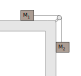
\includegraphics[width=0.6\textwidth]{carrucole.4.pdf}
\end{figure}

In the system shown above, the block of mass $M_1$, is on a rough horizontal table.

The string that attaches it to the block of mass $M_2$ passes over a frictionless pulley of negligible mass.

The coefficient of kinetic friction $\mu_k$ between $M_1$ and the table is less than the coefficient of static friction $\mu_s$.

\begin{enumerate}
\item On the diagram below, draw and identify all the forces acting on the block of mass $M_1$
\begin{figure}[h]
\centering
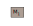
\includegraphics[width=0.4\textwidth]{carrucole.5.pdf}
\end{figure}
\item In terms of $M_1$ and $M_2$ determine the minimum value of $\mu_s$ that will prevent the blocks from moving

\vspace{1cm}
The blocks are set in motion by giving $M_2$ a momentary downward push.  In terms of $M_1$, $M_2$, $\mu_k$ and $g$, determine each of the following:

\item The magnitude of the acceleration of $M_1$
\item The tension of the string
\end{enumerate}

Soluzione a pagina \pageref{s_2pca}

\end{enumerate}

\subsubsection{Multiple choice} \label{q_mcmc}

Soluzioni a pagina \pageref{s_mcmc}

\begin{enumerate}


\item 

A ball is fastened to a string and is swung in a vertical circle. When the ball is at the
highest point of the circle its velocity and acceleration directions are:

\begin{figure}[H]
\centering
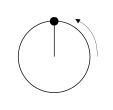
\includegraphics[width=0.4\textwidth]{rot-ex-1.pdf}
\end{figure}

\begin{figure}[h]

\centering

\begin{minipage}{.1\textwidth}
  \centering
  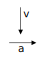
\includegraphics[width=\linewidth]{rot-ex-1a.pdf}
  A
\end{minipage}
\hspace{1cm}
\begin{minipage}{.1\textwidth}
  \centering
  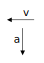
\includegraphics[width=\linewidth]{rot-ex-1b.pdf}
  B
\end{minipage}
\hspace{1cm}
\begin{minipage}{.1\textwidth}
  \centering
  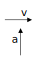
\includegraphics[width=\linewidth]{rot-ex-1c.pdf}
  C
\end{minipage}
\hspace{1cm}
\begin{minipage}{.1\textwidth}
  \centering
  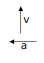
\includegraphics[width=\linewidth]{rot-ex-1d.pdf}
  D
\end{minipage}
\end{figure}

\item A ball with a mass m is fastened to a string and is swung in a vertical circle. 

(see previous picture for setup)

When the ball is at the highest point of the circle the tension in the string is:

\begin{itemize}
\item[A] $mg$
\item[B] $mg + ma$
\item[C] $ma ‐mg$ 
\item[D] $mg/ma$
\end{itemize}

\item An object, shown in the accompanying figure, moves in uniform circular motion.

Which arrow best depicts the net force acting on the object at the instant shown?

\begin{figure}[H]
\centering
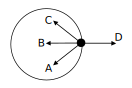
\includegraphics[width=0.4\textwidth]{rot-ex-3.pdf}
\end{figure}


\item A motorcyclist moves at a constant speed down one hill and up another hill along the smooth curved surface. 

\begin{figure}[H]
\centering
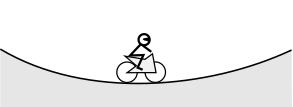
\includegraphics[width=0.6\textwidth]{mot-ex-4.pdf}
\end{figure}

When the motorcyclist reaches the lowest point of the curve its velocity and acceleration directions are:



\begin{figure}[H]

\centering

\begin{minipage}{.1\textwidth}
  \centering
  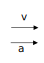
\includegraphics[width=\linewidth]{mot-ex-4a.pdf}
  A
\end{minipage}
\hspace{1cm}
\begin{minipage}{.1\textwidth}
  \centering
  \includegraphics[width=\linewidth]{mot-ex-4b.pdf}
  B
\end{minipage}
\hspace{1cm}
\begin{minipage}{.1\textwidth}
  \centering
  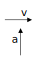
\includegraphics[width=\linewidth]{mot-ex-4c.pdf}
  C
\end{minipage}
\hspace{1cm}
\begin{minipage}{.1\textwidth}
  \centering
  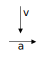
\includegraphics[width=\linewidth]{mot-ex-4d.pdf}
  D
\end{minipage}
\end{figure}

\item A car moves along the curved track. 

\begin{figure}[H]
\centering
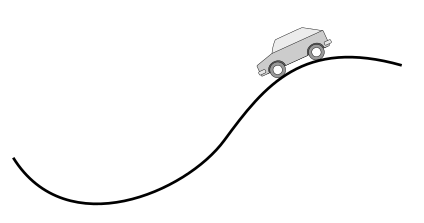
\includegraphics[width=0.6\textwidth]{rot-ex-4.pdf}
\end{figure}

What is the apparent weight of the driver when the car reaches the lowest point of the curve?

\begin{itemize}
\item[A] $mg$
\item[B] $mg+ma$
\item[C] $ma-mg$ 
\item[D] $mg/ma$
\end{itemize}

\item Acar moves along the curved track (same situation as the previous question).

What is the direction of $F_N$ of the driver when the car reaches the lowest point of the curve?

\begin{itemize}
\item[A] Upward
\item[B] Downward
\item[C] Forward
\item[D] Backward
\end{itemize}


\item A car is traveling on a road in hilly terrain, see figure above.
Assume the car has speed $v$ and the tops and bottoms of the hills have radius of curvature $R$.
The driver of the car is most likely to feel weightless:

\begin{itemize}
\item[A] at the top of a hill when $v = \sqrt{gR}$
\item[B] at the bottom of a hill when $v > \sqrt{gR}$
\item[C] going down a hill when $v = \sqrt{gR}$
\item[D] at the top of a hill when $v < \sqrt{gR}$
\end{itemize}

\vspace{1cm}

A 0.2 kg ball rotates at a constant speed of 3 $\frac{m}{s}$ on the end of 1.2 m long string.

The string describes a horizontal circle.

\begin{figure}[H]
\centering
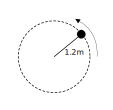
\includegraphics[width=0.3\textwidth]{rot-ex-5.pdf}
\end{figure}

\item What is the centripetal acceleration of the object?

\begin{itemize}
\item[A] $1.2 \frac{m}{s^2}$
\item[B] $3.0 \frac{m}{s^2}$
\item[C] $7.5 \frac{m}{s^2}$
\item[D] $3.2 \frac{m}{s^2}$
\end{itemize}


\item What is the centripetal force exerted on the object?

\begin{itemize}
\item[A] $1.0 N$
\item[B] $1.2 N$
\item[C] $0.2 N$
\item[D] $1.5 N$
\end{itemize}


\item When a student stands on a rotating table, the frictional force exerted on the student by the table is

\begin{itemize}
\item[A] greater in magnitude than the frictional force exerted on the table by the student
\item[B] less in magnitude than the frictional force exerted on the table by the student
\item[C] equal in magnitude than the frictional force exerted on the table by the student
\item[D] directed away from the center of the table
\end{itemize}


\item A child whirls a ball at the end of a rope, in a uniform circular motion. 

Which of the following statements is NOT true?

\begin{itemize}
\item[A] The speed of the ball is constant.
\item[B] The velocity of the ball is constant.
\item[C] The radius is constant
\item[D] The magnitude of the ball’s acceleration is constant.
\end{itemize}



\item The horizontal table rotates at a constant speed. 

As viewed from above, a coin on the table moves counterclockwise in a circle.



\begin{figure}[H]
\centering
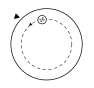
\includegraphics[width=0.4\textwidth]{rot-ex-12.pdf}
\end{figure}

Which of the following vectors best represents the direction of the frictional force 
exerted on the coin by the table when the coin is in the position shown?

\begin{figure}[H]

\centering

\begin{minipage}{.1\textwidth}
  \centering
  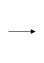
\includegraphics[width=\linewidth]{rot-ex-12a.pdf}
  A
\end{minipage}
\hspace{1cm}
\begin{minipage}{.1\textwidth}
  \centering
  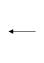
\includegraphics[width=\linewidth]{rot-ex-12b.pdf}
  B
\end{minipage}
\hspace{1cm}
\begin{minipage}{.1\textwidth}
  \centering
  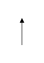
\includegraphics[width=\linewidth]{rot-ex-12c.pdf}
  C
\end{minipage}
\hspace{1cm}
\begin{minipage}{.1\textwidth}
  \centering
  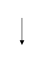
\includegraphics[width=\linewidth]{rot-ex-12d.pdf}
  D
\end{minipage}
\end{figure}

\item A centripetal force $F$ is applied to an eraser moving at a constant speed $v$ in a horizontal circle of radius $r$.

If the same force is applied, but the radius is halved, what happens to the speed of the eraser?

\begin{itemize}
\item[A] Increased by a factor of $2$
\item[B] decreased by a factor of $2$  
\item[C] increased by a factor of $\sqrt{2}$  
\item[D] decreased by a factor of $\sqrt{2}$
\end{itemize}

\item A centripetal force $F$ is applied to an object moving at a constant speed $v$
in a horizontal circle of radius $r$.

If the radius is quadrupled and the speed is doubled, what happens to the centripetal force?

\begin{itemize}
\item[A] Increased by a factor of $2$
\item[B] decreased by a factor of $2$
\item[C] doesn’t change
\item[D] increased by a factor of $\sqrt{2}$
\end{itemize}


The diagram below is a snapshot of three cars all moving counterclockwise during a 
one lap race on an elliptical track.  


\begin{figure}[H]
\centering
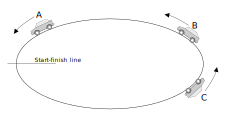
\includegraphics[width=0.6\textwidth]{rot-ex-15.pdf}
\end{figure}


\item Which car the moment of the snapshot has the smallest displacement?

\begin{itemize}
\item[A] car A
\item[B] car B
\item[C] car C
\item[D] all three cars have the same displacement 
\end{itemize}

\item Which car at the moment of the snapshot must have none zero acceleration?

\begin{itemize}
\item[A] car A
\item[B] car B
\item[C] car C
\item[D] all three cars have none zero acceleration
\end{itemize}


\item Which car can at the moment of the snapshot must have a centripetal force directed to the center of the center of the curvature?

\begin{itemize}
\item[A] car A
\item[B] car B
\item[C] car C
\item[D] all three cars must have the centripetal force directed to the center of the curvature
\end{itemize}


\item A roller coaster car is on a track that forms a circular loop of radius $R$ in the vertical plane.
If the car is to just maintain contact with track at the top of the loop, 
what is the minimum value for its velocity at this point? 

\begin{itemize}
\item[A] $gR$
\item[B] $0.5gR$
\item[C] $2gR$
\item[D] $(gR)^{\frac{1}{2}}$
\end{itemize}

\item A coin rests on a turntable a distance $r$ from the axis of rotation.
The turntable rotates with a constant speed of $v$.
What is the minimum coefficient of static friction between the turntable and the coin?

\begin{itemize}
\item[A] $v^2rg$
\item[B] $\frac{v^2}{rg}$
\item[C] $\frac{rg}{v^2}$
\item[D] $\frac{v^2}{r}$
\end{itemize}


\item A car goes around a curve of radius $r$ at a constant speed $v$.
The coefficient of static friction between the tires and the surface is $\mu$.
What is the maximum value of the car’s velocity in order to prevent car from skidding of the road? 
 
\begin{itemize}
\item[A] $\mu rg$
\item[B] $\frac{\mu r}{g}$
\item[C] ${\mu µrg}^2$
\item[D] $\frac{g}{\mu r}$
\end{itemize}



\end{enumerate}



\subsection{Gravitazione} \label{gravitazione}


\setcounter{equation}{0}
\begin{enumerate}

\item \label{grav_01}

Un satellite artificiale su un’orbita circolare si trova a un’altezza $h=600\:km$
dalla superficie della Terra, il cui raggio misura $R_T=6,37\times 10^3\: km$
e la cui massa vale $M=5,97\times 10^{24}\; kg$.

Calcolare:

\begin{enumerate}
\item la velocità $v$ con la quale il satellite ruota intorno alla Terra
\item la velocità angolare $\omega$ del satellite nel suo moto intorno alla Terra
\item il periodo di rivoluzione $T$
\end{enumerate}



( Soluzione a pagina \pageref{grav_s_01} )

\item \label{grav_02}

I satelliti geostazionari sono così chiamati perché rimangono sempre sulla verticale dello stesso punto della superficie terrestre.

Determina a quale altezza si trovano rispetto alla superficie del nostro pianeta.

Per risolvere il problema hai a disposizione queste formule:

\begin{enumerate}
\item Periodo di rotazione della Luna intorno alla Terra:
	\[T_L=2,36\times 10^6\:s\]
\item Raggio dell'orbita della Luna:
	\[R_L=3,84\times 10^5\:km\]
\item Periodo di rotazione della Terra:
	\[T_T=23,9\:h\]
\item Raggio della Terra:
	\[R_T=6,37\times 10^3\:km\]
\end{enumerate}

( Soluzione a pagina \pageref{grav_s_02} )


\end{enumerate}



\input{soluzioni.moto.lineare.tex}

\subsection*{Soluzioni di esercizi nella sezione ``\textbf{\nameref{carrucole}}".}

Soluzione dell'esercizio \ref{car_x_01} a pagina \pageref{car_x_01}\label{car_s_01}

\begin{figure}[h]
\centering
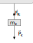
\includegraphics[width=0.2\textwidth]{fili_01_01.pdf}
\end{figure}

Sul corpo agiscono due forze.
\begin{enumerate}
\item[$\vec{P}_c$] : la forza peso del corpo stesso 
\item[$\vec{F}_{fc}$]: la forza esercitata dal filo sul corpo
\end{enumerate}

\[ \vec{F}_{tot} = \vec{P}_c+\vec{F}_{fc} \]

La fune esercita la sua forza nel punto di contatto con il corpo.

È possibile considerare il corpo come se fosse un unico punto: il centro di massa
del corpo, dove agiscono tutte le forze.

Il corpo è a riposo quindi la forza totale che agisce su esso è nulla: 
\[ \vec{f}_{tot} = 0 N \]
Ne consegue che:
\[  \vec{P}_c = -\vec{F}_{fc} \]
\[ | \vec{P}_c | =  |\vec{F}_{fc} | = m_cg =7kg\cdot 9.81 \frac{m}{s^2} = 69N \]

Terzo principio della dinamica: la forza $\vec{F}_{fc}$ esercitata dal filo sul 
corpo è uguale e contraria alla forza $\vec{F}_{cf}$, esercitata dal corpo sul filo
,che è la grandezza da trovare.

\begin{figure}[h]
\centering
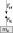
\includegraphics[width=0.1\textwidth]{fili_01_02.pdf}
\end{figure}

\[ \vec{F}_{cf} = - \vec{F}_{fc} \]
\[ | \vec{F}_{cf} | = | \vec{F}_{fc} | = 69 N \]

Il soffitto, anch’esso in quiete, esercita una forza $\vec{F}_{sf}$
uguale e contraria alla forza $\vec{F}_{fs}$ che il filo esercita sul soffitto.

\begin{figure}[h]
\centering
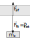
\includegraphics[width=0.2\textwidth]{fili_01_03.pdf}
\end{figure}

Questa forza $\vec{F}_{fs}$ è uguale alla forza $\vec{P}_{tot}$
determinata dal peso del corpo e del filo, ma con un punto di applicazione
diverso.
\[ - \vec{F}_{sf} = \vec{F}_{fs} = \vec{P}_{tot} \]
\[ \vec{P}_{tot} = \vec{P}_c + \vec{P}_f \]
\[ |\vec{F}_{sf}| = |\vec{P}_{tot} = | \vec{P}_c | + | \vec{P}_f  | = m_cg+m_fg= \]
\[ (7 kg + 50 g) \cdot 9.81 \frac{m}{s^2} = (7 kg + 0,05 Kg) \cdot 9.81 \frac{m}{s^2}
= 69.2 N \]





\vspace{1cm}
\hrule
\vspace{1cm}

Soluzione dell'esercizio \ref{ex_p_1} a pagina \pageref{ex_p_1}\label{sol_p_1}

If there were no gravity, in $1.5$ seconds the ball would have a displacement of
magnitude $12 \cdot 1.5$, that is $18 m$, at $70\circ$ to the horizontal.

This is represented by the arrow $\overrightarrow{OA}$ in the figure.

\begin{figure}[H]
\centering
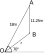
\includegraphics[width=0.3\textwidth]{ex_p_1.pdf}
\end{figure}

To this must be added a displacement of magnitude 

\begin{equation*}
\frac{1}{2}\cdot 10 \cdot 1.5m^2
\end{equation*}

that is $11.25 m$, vertically downwards, represented by the arrow AB.

The sum of these is the displacement OB.

So after 1.5 seconds the ball is at B.

\vspace{1cm}
\hrule
\vspace{1cm}

\begin{minipage}{\textwidth}
Soluzione dell'esercizio \ref{ex_p_2} a pagina \pageref{ex_p_2}\label{sol_p_2}

\begin{figure}[H]
\centering
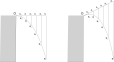
\includegraphics[width=0.8\textwidth]{ex_p_2.pdf}
\end{figure}

These diagrams were produced by superimposing several diagrams like
those in exercise \ref{ex_p_1}, but at intervals of $0.5s$ that is for

\begin{equation*}
t=0.5,1,1.5,\ldots,n
\end{equation*}


The displacements $\vec{u}t$ in these times have magnitudes $9 m$, $18 m$, $\ldots$.

The vertical displacements have magnitudes $1.25 m$, $5 m$, $11.25 m$, $\ldots$

The points corresponding to $A$ and $B$ at time $t$ are denoted by $At$ and $Bt$.

You can now show the paths by drawing smooth curves through the points $O$,
$B_{0.5}, B_{1}, \ldots$
for the two initial velocities.

\end{minipage}
\vspace{1cm}
\hrule
\vspace{1cm}

Soluzione dell'esercizio \ref{ex_p_3} a pagina \pageref{ex_p_3}\label{sol_p_3}


It is simplest to take the origin at ground level, rather than at the point
from which the ball is served, so add 2 to the $y$-coordinate given by the
general formula. 

If the initial speed of the ball is $p\frac{m}{s}$,


\begin{equation*}
x = pt \textrm{ and }y = 2 - 5t^2
\end{equation*}

Both conditions involve both the $x$- and $y$-coordinates, and the time $t$ is
used as the link.

The ball passes over the net when $12 = pt$, that is $t=\frac{12}{p}$

The value of $y$ is then

\begin{equation*}
2-5\left(
\frac{12}{p}
\right)=2-\frac{720}{p^2}
\end{equation*}

and this must be more than $0.9$, so 

\begin{equation*}
2-\frac{720}{p^2} > 0.9
\end{equation*}

This gives

\begin{equation*}
\frac{720}{p^2} <1.1
\end{equation*}


\begin{equation*}
p>\sqrt{\frac{720}{1.1}}\approx25.6
\end{equation*}

Considering the second constraint: the ball lands when $y = 0$, that is when 
$2 - 5t^2 = 0$, or 


\begin{equation*}
t=\sqrt{\frac{2}{5}}
\end{equation*}

It has then gone a horizontal distance of $p\sqrt{\frac{2}{5}}$
metres, and to satisfy the second condition you need $p\sqrt{\frac{2}{5}} < 18$.

This gives 



\begin{equation*}
p<18\sqrt{\frac{5}{2}}\approx 28.5
\end{equation*}


So the ball can be hit with any speed between about $25.6 \frac{m}{s}$
and
$28.5\frac{m}{s}$

\vspace{1cm}
\hrule
\vspace{1cm}

Soluzione dell'esercizio \ref{ex_p_4} a pagina \pageref{ex_p_4}\label{sol_p_4}

Known variables:

\begin{itemize}
\item[$s$] = $1.25m$
\item[$a$] = $9.81\frac{m}{s}$
\item[$u$] = 0
\item[$t$] = ?
\end{itemize}

The equations linking those variables are:


\setcounter{equation}{0}
\begin{equation}
s=ut+\frac{1}{2}at^2
\end{equation}

\begin{equation*}
s=\frac{1}{2}gt^2
\end{equation*}



\begin{equation*}
t=\sqrt{\frac{2s}{g}}
\end{equation*}


\begin{equation*}
t=\sqrt{
\frac{
2\cdot 1.25
}{
9.81
}
}=0.5s
\end{equation*}

Now consider the horizontal motion.

\begin{itemize}
\item[$s$] = $10m$
\item[$a$] = $0$
\item[$t$] = 0.5s
\item[$u$] = ?
\end{itemize}



\begin{equation*}
\textrm{velocity}
=\frac{
\textrm{displacement}
}{
\textrm{time}
}
\end{equation*}



\begin{equation*}
v=\frac{10}{0.5}=20\frac{m}{s}
\end{equation*}



\vspace{1cm}
\hrule
\vspace{1cm}




Soluzione dell'esercizio \ref{ex_2pca} a pagina \pageref{ex_2pca}\label{sol_2pca} \label{s_2pca}

\begin{enumerate}
\item All the forces acting on the block of mass $M_1$:

\begin{figure}[h]
\centering
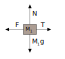
\includegraphics[width=0.4\textwidth]{carrucole.6.pdf}
\end{figure}

\begin{itemize}
\item[$M_1g$] è la \textbf{forza peso} 
\item[$N$] è la \textbf{reazione vincolare} del piano, reazione del piano stesso alla forza peso che impedisce al corpo di cadere attraverso il piano
\item[$T$] è la tensione esercitata dalla fune
\item[$F$] è la \textbf{forza d’attrito dinamico} o \textbf{statico}, a seconda che il corpo sia in quiete o in movimento.
\end{itemize}

\item 
La tensione della fune è pari alla forza esercitata dalla gravità su $M_2$:
\begin{equation*}
T=m_2g
\end{equation*}

Questo valore deve essere equivalente alla forza d'attrito dinamico:

\begin{equation*}
T=f_{max}=\mu_sm_1g
\end{equation*}

\begin{equation*}
\mu_sm_1g=m_2g
\end{equation*}

\begin{equation*}
\mu_s=\frac{m_2}{m_1}
\end{equation*}

\end{enumerate}

Soluzioni degli esercizi multiple choice da pagina \pageref{q_mcmc} \label{s_mcmc}

\begin{enumerate}
\item B
\item C
\item B
\item C
\item B
\item A
\item C
\item C
\item D
\item C
\item B
\item C
\item D
\item C
\item A
\item D
\item D
\item D
\item B
\item C
\item A
\item D
\item C
\item A, B
\item B, C
\end{enumerate}



\vspace{1cm}
\hrule
\vspace{1cm}


Soluzione dell' esercizio \ref{motocirc_e_00} a pagina \pageref{motocirc_e_00} \label{motocirc_s_00}

La risposta corretta è la ``C".

Un corpo che si muove su una traiettoria curva possiede in generale una componente
dell’accelerazione tangenziale, ossia diretta lungo la tangente alla traiettoria, responsabile
della variazione in modulo della velocità, ed una componente normale, diretta in direzione
radiale rispetto alla traiettoria e verso il centro della curva; essa è responsabile della varia-
zione in direzione della velocità. In un moto uniforme (velocità in modulo costante) la
componente tangenziale è nulla, per cui nel caso in esame è presente solo l’accelerazione
normale. 



\subsection*{Soluzioni di esercizi nella sezione ``\textbf{\nameref{gravitazione}}".}

Soluzione dell'esercizio \ref{grav_01} a pagina \pageref{grav_01}\label{grav_s_01}

Sappiamo che la formula che descrive la velocità di un satellite in orbita circolare è 
\[v=\sqrt{GM\over r}\]
da cui
\[v=\sqrt{6,67\times 10^{-11}\: N\cdot m^2/kg^2\times 5,97\times 10^{24}\; kg \over 600\times 10^3\:m+6,37\times 10^6\:m}\approx 7,56\times 10^3\;m/s\]

Per calcolare la velocità angolare ci ricordiamo che la relazione che lega la velocità angolare e la velocità tangenziale è

\[\omega={v\over r}={7,56\times 10^3\;m/s \over 600\times 10^3\:m+6,37\times 10^6\:m }\approx 1,08\times 10^{-3}\:rad/s\]

Infine calcoliamo il periodo di rivoluzione
\[T={2\pi r\over v}={2\pi\cdot (600\times 10^3\:m+6,37\times 10^6\:m)\over 7,56\times 10^3\;m/s }\approx 5,8\times 10^3\:s\]



Soluzione dell'esercizio \ref{grav_02} a pagina \pageref{grav_02}\label{grav_s_02}


Sappiamo che la Terra ha un periodo di rotazione di \[T_T=23,9\:h\]
se vogliamo che il satellite sia sempre sulla verticale dello stesso punto necessitiamo che i due periodi siano uguale, ossia 

\[T_s=T_T\]

\[{2\pi\cdot r_s\over v_s}=T_T\]

\[{2\pi\cdot r_s\over \sqrt{GM_T/r_s}}=T_T\]

\[{2\pi\cdot \sqrt {r_s^3}\over \sqrt{GM_T}}=T_T\]

\[\sqrt {r_s^3}={\sqrt{GM_T}\cdot T_T\over 2\pi}\]

\[r_s=\sqrt[3]{GM_T\cdot T_T^2\over 4\pi^2}\]

Per terminare ci basta ricavare la massa terrestre. Sappiamo che


\[T_L={2\pi\cdot R_L\over v_L}={2\pi\cdot r_L\over \sqrt{GM_T/r_L}}\Rightarrow M_T={4\pi^2R_L^3\over GT_L^2}\]

da cui, sostituendo nella formula scritta sopra

\[r_s=\sqrt[3]{GM_T\cdot T_T^2\over 4\pi^2}=\sqrt[3]{G\cdot 4\pi^2\cdot R_L^3\cdot T_T^2\over 4\pi^2\cdot GT_L^2}=\sqrt[3]{ R_L^3\cdot T_T^2\over T_L^2}\]

e pertanto

\[r_s=\sqrt[3]{ (3,84\times 10^8\:m)^3\cdot (23,9\cdot 3600\:s)^2\over (2,36\times 10^6\:s)^2}\approx 4,22\times 10^7\: m\]

Pertanto l’altezza a cui dovrà stazionare il satellite sarà


\[h_s=r_s-R_T=4,22\times 10^7\:m-6,37\times 10^6\:m\approx 3,58\times 10^7\:m\]




% \end{NoHyper}
\end{document}

